\chapter{Higher Order Applications: Multiple Object Tracking}

As the final aim of my thesis, I am going to inspect the performance of the chosen object detectors on a higher-order problem, namely multiple object tracking. First I am going to review the problem itself, and the common metrics used to measure its performance. 

After this, I will elaborate on the object tracking method I chose as the basis, showing how it incorporates the aforementioned detectors, and the way the performance of the latter is expected to influence tracking performance.

\section{The problem and possible approaches}

Multiple object tracking (MOT) consists of determining the \textit{trajectory} of given kinds of objects in a video stream. In the current context, the trajectory of a single, unique object is a series of bounding boxes with an identifier, one box for every frame in which the object is visible. The rectangular bounding boxes are expected to fit the object shilouette as tightly as possible.

Along the years, several approaches have been developed for the problem, but with the advent of highly accurate object detectors (most notably the breakthrough of convolutional neural networks from the mid-2010s and onward), the detection-based paradigm has become one of the most popular.

The approach consists of detecting objects on each new frame, then assigning them to previously found trajectories, if the object has been seen before, or registering a new trajectory otherwise. This is generally called the \textit{association step}. In some scenarios, when the objects of interest are densely packed, this can pose a considerable difficulty.

Among some popular solutions to this association problem are the \textit{proximity-based} (the Simple Online and Realtime Tracking (SORT) architecture~\cite{Bewley_2016} is one example) and the \textit{feature-based} (the DeepSORT architecture \cite{DeepSORT} incorporates such methods using \textit{deep appearance descriptors}) assignments. The former considers each already existent trajectory, takes their previous location, or the predicted location for this time step, and does the assignment based on some spatial distance between these and current detections. The latter does overarching associations based on visual appearance features, not necessarily restricted to the appearance observed in the last few frames.

The weakness of the proximity-based approach is when the density of objects is high, their movement highly dynamic and their trajectories intertwined. In this case, feature-based methods might excel. The weakness of the feature-based methods might show when they confuse similar, but distinct objects, or when they cannot account for some drastic, fast changes in appearance (like changes in lighting, orientation, deforming, or partial occlusion). In these situations, assignment to last known locations can help. Thus, these two approaches are not, and should not be exclusive.

The introduction above focuses on paradigms and aspects mostly relevant for my thesis, and narrows down the field somewhat. For a comprehensive, recent overview of the problem, see the literature review at~\cite{Luo_2021}. It goes beyond just the detection-based approach, and also formalises the general problem.

Finally, it is worth mentioning that the most common multi-object tracking targets are pedestrians, faces and vehicles, and thus most popular MOT datasets consist of these. In this thesis, I am going to tackle tracking vehicles in road traffic footages.

\section{Metrics}

The MOT challenge~\footnote{\url{https://motchallenge.net/}} is one of the most popular currently used multiple object tracking benchmarks. Its most recent version is the MOT20 benchmark.

\section{SORT}

\textbf{TODO: explain SORT}

\section{My measurement}
\subsection{Data}

I will evaluate the model's performance for multi-object tracking on the UA-DETRAC dataset\footnote{\url{https://detrac-db.rit.albany.edu/}}. The dataset contains 100 videos (60 for training, 40 for testing) of road traffic captured at different locations in China. The total length of the video footage is around 10 hours, stored frame by frame (as separate 960 pixel by 540 pixel JPEG images), at the rate of 25 frames per second.

The annotations contain information about vehicle type, illumination, scale (proportional to the square root of the bounding box area), occlusion ratio (the measure by which other objects occlude the vehicle) and truncation ratio (the degree of the bounding box lying outside the frame). Information about weather conditions e.g.~rainy, cloudy, sunny etc.~is also included.

\subsection{Benchmark}

The dataset and the benchmark is described in~\cite{CVIU_UA-DETRAC}. The article also proposes an evaluation protocol for multi-object tracking. A key point is the joint analysis of detection and tracking performance, analysing the effects of the chosen model's precision/recall values (and the underlying confidence threshold setting that influences both) in relation with the tracking performance, as reflected by the MOTA and MOTP score. These relationships are visualized on the PR-MOTA and PR-MOTP curves (See figure \ref{fig:pr-mota}).

\begin{figure}[h]
    \captionsetup{width=\textwidth}
    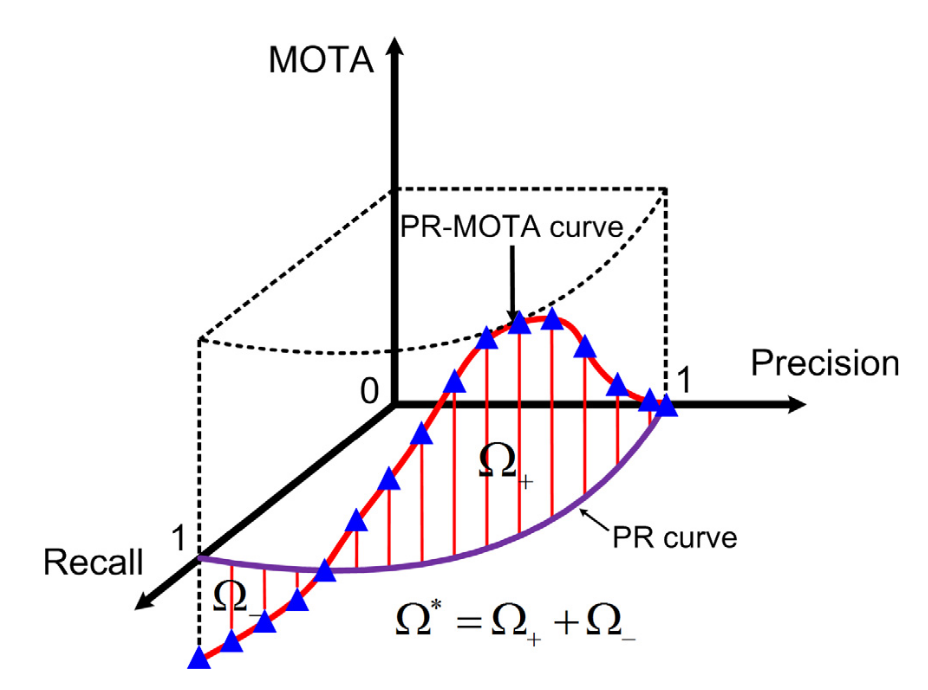
\includegraphics[width=\textwidth]{figures/pr-mota-curve.png}
    \caption{Visualization of the PR-MOTA curve. Image taken from \cite{CVIU_UA-DETRAC}}
    \label{fig:pr-mota}
\end{figure}

The authors argue that, as it is not fair, nor enough to compare the performance of two object detectors based on different points on the PR curve, it is also not enough to determine the maximum point on the PR-MOTA curve, as a good tracker must produce good scores in a wider range of settings. The whole range of the curve must be taken into account in some form, thus the need for a new metric, $\Omega^{*}$, or the \textit{PR-MOTA score}:

\[ \Omega^{*} = \frac{1}{2}\int_{\mathcal{C}} \Psi(p, r) \,d\textbf{s} \]

where $\Psi$ is the MOTA score across the whole dataset at precision $p$ and recall $r$, and we calculate the (approximate value of the) signed area under the PR-MOTA curve as an integral along the PR curve $\mathcal{C}$ (for every $(p, r) \in \mathcal{C}$). Dividing by 2 ensures that the score stays in the interval $(-\infty, 100\%]$. Similar metrics can be defined for the MOTP, FP, FN, IDS, MT and ML scores.

\textbf{TODO: explain MOTA, MOTP, FP, FN, IDS, MT, ML}.

\subsection{Evaluation}

The tracking evaluation toolkit on the official DETRAC website is not available\footnote{\url{https://detrac-db.rit.albany.edu/Tracking}, under DETRAC-toolkit (Windows beta)}, because the login feature does not work. Thus, I had to write my own implementation for the evaluation based on the CLEAR MOT metrics~\cite{Bernardin2008}.

\subsection{Data Exploration}

At the time of writing this thesis, the test and train images, grouped into sequences that form videos, can be accessed through the Download page of the official site\footnote{\url{https://detrac-db.rit.albany.edu/download}} as \verb|DETRAC-train-data.zip|. However, the tracking annotations for the train and test sets cannot be downloaded, as clicking on the links triggers a popup prompting to log in first. As the login functionality currently does not work, I had to look for alternative ways to access the data.  

Fortunately, after a short search I have found a GitHub repository owned by the Georgia Tech Database Group. Their Exploratory Video Analytics System (EVA) repository contains, among others, a guide on how to download the UA-DETRAC dataset\footnote{\url{https://github.com/georgia-tech-db/eva/tree/master/data/ua_detrac}}, along with a bash script serving the same purpose.

Through those links, I could download the training annotations. Sadly, the test annotations, claimed on the official UA-DETRAC website to be released, were still nowhere to be found, but I figured the 60 sequences (or even a subset of them) should be enough to evaluate tracking performance. The integrity of the measurement wouldn't have been compromised either, as I wasn't planning on doing detector training or hyperparameter tuning on the train set. There were two kinds of training annotation formats provided: XML and MAT.

The XML annotations are meant for detection training, and contain additional information like vehicle category, weather conditions during filming and bounding box scale. I did not use this data directly, as I used the models pre-trained on the COCO dataset, but inspecting this data confirms the vehicle categories supported by the DETRAC dataset: \textit{car}, \textit{van}, \textit{bus}, \textit{other}. The corresponding COCO object categories are \textit{car}, \textit{truck}, \textit{bus}, so that is what I will be looking for when runnning detection on the images, and ignoring all other classes.

The MAT annotations are files in MATLAB serialization format, containing trajectory and position information for all tracked entities. For every image sequence, there is a \verb|MVI_NNNNN.MAT| file.
The image sequences themselves are consecutive frames under \verb|Insight-MVT_Annotation_Train/MVI_NNNNN|, after unzipping \verb|DETRAC-train-data.zip|.

Initially I inspected the MAT files' inner structure (see figure~\ref{fig:octave-exploration}) in GNU Octave, MATLAB's open-source and somewhat compatible counterpart. I found that each file contained 5 matrices:
\begin{enumerate}
    \item{$X$: An $N \times T$ matrix, where $T$ is the number of trajectories, and $N$ is the number of frames. Given the frame $i$ and trajectory $j$, $x_{i,j}$ denotes the $x$ coordinate of the bottom center of the bounding box\footnote{I found this out initially through trial and error, when trying to visualize bounding boxes in Python, because I did not know this to be a common format for specifying bounding boxes. Later, I found it mentioned in \url{https://detrac-db.rit.albany.edu/FAQ} as \textit{foot position}.}, or $0$ if trajectory $j$ is not present in that frame.}
    \item{$Y$: An $N \times T$ matrix, similar to $X$, but it contains the $y$ coordinates of the bounding boxes' foot position.}
    \item{$W$: contains the width of the boxes.}
    \item{$H$: contains the height of the boxes.}
    \item{$frameNums$: A row vector of length $N$, containing the 1-based indices of the frames.}
\end{enumerate}

\begin{figure}[h]
    \begin{center}
        \captionsetup{width=0.8\textwidth}
        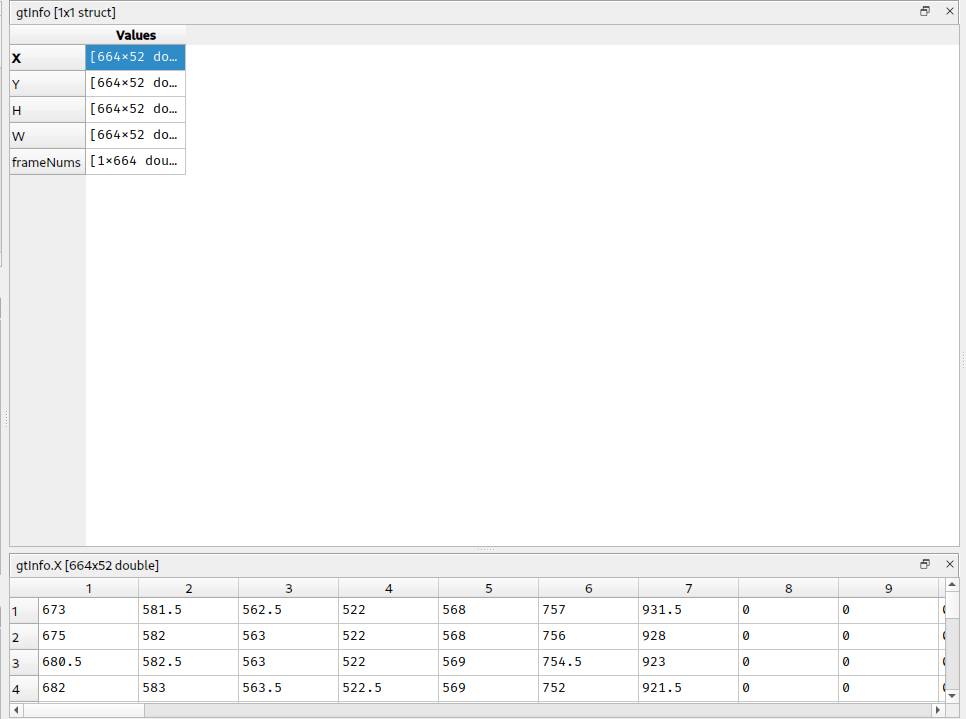
\includegraphics[width=0.8\textwidth]{figures/octave.png}
        \caption{Label data exploration in octave}
        \label{fig:octave-exploration}
    \end{center}
\end{figure}

\subsection{Data Processing}

...



% \subsection{Rest}

% Usually, a baseline for detection performance in MOT is the R-CNN architecture and its variants.

% For the MOT task, I have chosen the SORT architecture, introduced in~\cite{Bewley_2016}. Altough not the most recent, it is the architecture I have examined in my project laboratory, and has the analytical advantage of solely relying on detection performance, as opposed to method like DeepSORT that are influenced by the association method as well. It can be considered a reasonable baseline methood, relying on first-order velocity estimation and smoothing measurement errors based on the Kalman Filter.  